\documentclass[%
aps, pre,
amsmath,amssymb,
reprint,%
%author-year,%
% author-numerical,%
%superscriptaddress,
%showpacs, showkeys,
]{revtex4-1}

\usepackage{trinhcmd}
\usepackage{microtype}
\usepackage{graphicx}% Include figure files
\usepackage{rotating}
\usepackage{dcolumn}% Align table columns on decimal point
\usepackage{bm}% bold math
\usepackage{color}
% \usepackage{amsmath, amsthm, amssymb}
\usepackage{upgreek}
\usepackage{natbib}
\usepackage[pdfauthor={Philippe H. Trinh}]{hyperref}
\usepackage[inactive, tightpage]{preview}

\DeclareMathOperator{\Div}{div}
\DeclareMathOperator{\trace}{trace}
\DeclareMathOperator{\cp}{cp}
\DeclareMathOperator{\ecp}{ecp}
\DeclareMathOperator{\sd}{sd}
\DeclareMathOperator{\curl}{curl}
\DeclareMathOperator{\id}{id}
\DeclareMathOperator{\codim}{codim}
\DeclareMathOperator{\spa}{span}
\DeclareMathOperator{\argmin}{\arg\min}

\newcommand{\surf}{\mathcal{S}}
\newcommand{\band}{B(\surf)}

\newcommand{\lap}{\Delta}
\newcommand{\grad}{\nabla}
\newcommand{\sgrad}{\grad_{\surf}}
\newcommand{\slap}{\sgrad^2}
\newcommand{\sDiv}{\Div_{\surf}}
\newcommand{\sInt}{\int\limits_{\surf}}

\newcommand{\dx}{h}
\newcommand{\dt}{\tau}

% Mathematical constants
\newcommand{\ep}{\epsilon}
\newcommand{\Real}{\mathbb{R}}

\newcommand{\todo}[1]{\textbf{\textcolor{blue}{TODO: #1}}}
\newcommand{\tens}[1]{\mathbf{#1}}

\newtheorem{theo}{Theorem}[section]
\newtheorem{defi}[theo]{Definition}
\newtheorem{principle}[theo]{Principle}
\newtheorem{cor}[theo]{Corollary}
\newtheorem{lem}[theo]{Lemma}
\newtheorem{prop}[theo]{Proposition}

% Vectors
\newcommand*{\x}{\bm{x}}
\newcommand*{\xhat}{\hat{\bm{x}}}
\newcommand{\ea}{\hat{\bm{e}}_1}
\newcommand{\eb}{\hat{\bm{e}}_2}
\newcommand{\ec}{\hat{\bm{n}}}
\newcommand{\ek}{\hat{\bm{e}}_k}
\newcommand*{\n}{\mb{n}}
\newcommand*{\hatg}{\hat{\mb{g}}}
\renewcommand*{\r}{\mb{r}}

% Physical constants
\renewcommand*{\Rey}{\mathrm{Re}}
\newcommand*{\Bo}{\mathrm{Bo}}
\newcommand*{\Cn}{\mathscr{C}}
\newcommand*{\Bn}{\mathscr{B}}

\newcommand*{\rs}{\bm{R}}
\newcommand*{\K}{\mathcal{K}}
\newcommand*{\E}{\mathrm{E}}
\newcommand*{\F}{\mathrm{F}}
\newcommand*{\G}{\mathrm{G}}
\renewcommand*{\L}{\mathrm{L}}
\newcommand*{\M}{\mathrm{M}}
\newcommand*{\N}{\mathrm{N}}
\newcommand*{\Q}{\bm{Q}}
\renewcommand{\t}[1]{\tilde{#1}}

\newcommand*{\dsa}{\operatorname{\partial_{s_1}\!}}
\newcommand*{\dsb}{\operatorname{\partial_{s_2}\!}}
\newcommand*{\dsaa}{\operatorname{\partial_{s_1}^2\!}}
\newcommand*{\dsab}{\operatorname{\partial_{s_1 s_2}^2\!}}
\newcommand*{\dsbb}{\operatorname{\partial_{s_2}^2\!}}

\renewcommand{\ol}[1]{\overline{#1}}



\begin{document}

\preprint{Draft Version}

\title[Thin films on curved surfaces]{Thin film flows on general curved surfaces with gravity and surface tension}

\author{Colin B.~Macdonald}%
\affiliation{Oxford Centre for Collaborative and Applied Mathematics, Mathematical Institute, University of Oxford, Oxford OX2 6GG, UK}
\author{Thomas M\"{a}rz}%
\affiliation{Oxford Centre for Collaborative and Applied Mathematics, Mathematical Institute, University of Oxford, Oxford OX2 6GG, UK}
\author{Philippe H. Trinh}%
\thanks{Corresponding author: trinh@maths.ox.ac.uk}
\affiliation{Oxford Centre for Industrial and Applied Mathematics, Mathematical Institute, University of Oxford, Oxford OX2 6GG, UK}

\date{\today}

\begin{abstract}
We present a numerical study of gravity-driven thin film flows on curved surfaces including the effects of surface tension. We are particularly motivated by the aspect of gravity-driven fingering instabilities. 
\end{abstract}


\pacs{}% PACS
\keywords{thin film dynamics, closest point method, surface-intrinsic differential equations}%Use showkeys class option if keyword
\maketitle

\section{Introduction}\label{sect:Intro}

There is much interest in the study of thin film dynamics on general curved surfaces. In comparison with problems on flat surfaces, the main challenge is to propose a convenient three-dimensional coordinate system for its study. Even once such a coordinate system has been established, there are notable challenges, particularly in regards to surfaces with removable coordinate singularities.

Much of the research is based on surfaces that are easily parameterized: cylinders, tori. 

Many physical problems of interest:
\begin{enumerate}
\item Work of Mayo et al \cite{mayo_2013} on gravity-driven instabilities
\item Work of Trinh\cite{trinh_2014}, Lister, etc. on Rayleigh-Taylor instability
\item Work of Takagi and Huppert \cite{takagi_2010} on gravity-driven flow on a sphere
\end{enumerate}

\section{Thin film equations}

\noindent We consider the flow of a viscous, incompressible fluid on the surface of a two-dimensional solid substrate, $\mathcal{S} \subset \mathbb{R}^3$, under the influence of gravity and surface tension (Fig.~\mbox{[---]}). In this section, we shall recapitulate the essential details behind the derivation of the lubrication equations on general surfaces. Our equations follow from a combination of Howell~\cite{howell_2003} and \citeauthor{myers_2002}~\cite{myers_2002}, but makes a small correction to the free-surface curvature in the latter work. Additional details concerning the differential geometry can also be found in the work by \citeauthor{roy_2002}~\cite{roy_2002}. 

\subsection{Parameterization and non-dimensionalization}

Every point on the surface, $\mathcal{S}$, is characterized by a normal vector $\mb{n}$, and two principal curvatures, denoted $\kappa_1$ and $\kappa_2$, with $\kappa_1 \leq \kappa_2$. We define a mapping from the Cartesian $(x,y,z)$ system to an orthogonal curvilinear coordinate system given by $(s_1, s_2, s_3)$, where $s_1$ and $s_2$-curves are lines of constant principal curvature, and $s_3$ is distance measured in the normal direction from the surface. If $\mb{e}_1$, $\mb{e}_2$, and $\bm{n}$ respectively denote the unit orthogonal vectors for the coordinate system, then a general point in space is given by the position vector
\begin{equation} \label{rvec}
\mb{r}(s_1, s_2, s_3) = \rs(s_1, s_2) + s_3 \bm{n},
\end{equation}
%
where the surface is given by $\rs= \rs(s_1, s_2)$, and the fluid surface is given by $s_3 = h(s_1, s_2, t)$. Note that the parameterization by the lines of constant curvature is particularly convenient for the derivation, but once the governing equations have been derived with surface operators, other coordinate systems can be used. 

We assume that the velocity field of the fluid is given by $\mb{u} = u_1 \ea + u_2 \eb + u_3 \ec$, and take advantage of the thin-film approximation using the following non-dimensionalization:
\begin{equation}\label{nondim}
\begin{gathered}
\left[s_1\right] = \left[s_2\right] = L, \ [s_3] = \delta L, \\
[\kappa_1] = [\kappa_2] = 1/L, \\
[u_1] = [u_2] = U, \ [u_3] = \delta U, \\ 
[p] = \mu U/(\delta^2 L), \ [t] = L/U.
\end{gathered}
\end{equation}
%
Our key assumption is that the aspect ratio of the thin film is small, with $\delta \ll 1$. Notice that different from Howell~\cite{howell_2003}, we have chosen to scale the principal curvatures, $\kappa_1$ and $\kappa_2$ using the spatial scaling, $L$ (rather than introduce a separate curvature scale). In this work, we shall proceed with the assumption that $\kappa_i = \Oh(1)$, but but this may not always hold (e.g. near a sharp corner). The velocity scales are chosen according to the continuity equation, and the pressure scale is the typical slow-flow scaling so as to balance the viscous contributions. In what follows, we shall assume that all quantities have been non-dimensionalized according to \ref{nondim}.

In order to characterize the distances and shapes of the substrate, $\rs$, and free surface, $\r$ with $s_3 = h$, we require the specification of the first and second fundamental forms. For the substrate, these are $\{\E, \F, \G, \L, \M, \N\}$, defined in \eqref{funform}, and with tildes using same notation for the free-surface quantities. We can verify that the metric coefficients are, 
\begin{equation} \label{mcoef}
\begin{split}
m_1^2 &= \|\r_1 \|^2 = \E(1 - \ep h \kappa_1)^2 + \Oh(\ep^2) \\
m_2^2 &= \|\r_2 \|^2 = \G(1 - \ep h \kappa_2)^2 + \Oh(\ep^2) \\
m_3^2 &= \|\r_3 \|^2 = \ep^2.
\end{split}
\end{equation}
%
where $a_1 = \|\rs_1\| = \sqrt{\E}$ and $a_2 = \|\rs_2\| = \sqrt{\G}$ are the metric coefficients for the substrate. For a given substrate geometry, once the metric coefficients are known, the vector operators such as the divergence, gradient, and curl can be calculated. 
	
\subsection{Lubrication equations}

In this work, we assume that the fluid satisfies a no-flux and zero-slip conditions on the solid substrate. On the free surface, $s_3 = h(s_1, s_2, t)$, the fluid satisfies the kinematic and dynamic conditions. In total, 
\begin{subequations}
\begin{align}
u_1, u_2, u_3 = 0
&\quad \text{on $s_3 = 0$} \label{zeroslip} \\
u_1, u_2 = \Oh(\delta)  
&\quad \text{on $s_3 = h$} \label{tanstress} \\
u_3 = \pd{h}{t} + \frac{u_1}{m_1} \pd{h}{s_1} + \frac{u_2}{m_2} \pd{h}{s_2} 
&\quad \text{on $s_3 = h$} \label{kinematic} \\
\Delta p =  -\Cn \K + \Oh(\delta^2) 
&\quad \text{on $s_3 = h$} \label{psurf}
\end{align}
\end{subequations}
%
where $\Delta p$ is the jump in the pressure across the free surface, $\K$ is twice the mean curvature and $\Cn = \gamma \delta^2/(\mu U)$ is an inverse Capillary number.

We integrate the continuity equation, $\nabla \cdot \mb{u} = 0$, over the thin film, and combine with the substrate \eqref{zeroslip} and kinematic \eqref{kinematic} conditions to give the following conservation equation for the flux
\begin{subequations}
\begin{equation}
a_1 a_2 \pd{h}{t} + \pd{Q_1}{s_1} + \pd{Q_2}{s_2} = \Oh(\delta),
\end{equation}
%
applied on $s_3 = h$, and where the fluxes are given by 
\begin{equation} \label{flux1}
Q_k = \int_0^h a_k' u_k \, \de{s_3} + \Oh(\delta)
\end{equation} 
\end{subequations}
%
and $a_1' = a_2$ and $a_2' = a_1$. Notice the neglected terms in the above expressions arise due to an approximation of the free-surface metric coefficients $m_i$ using the metric coefficients of the substrate.

The non-dimensionalized slow flow equations are
\begin{subequations} \label{stokes}
\begin{align}
\frac{1}{a_k} \pd{p}{s_k} &= \pdd{u_k}{s_3} + B (\hat{\mb{g}} \cdot \ek) + \Oh(\delta, \delta^2\Rey), \label{stokes12} \\
\pd{p}{s_3} &= \delta \Bn (\hat{\mb{g}} \cdot \ec) + \Oh(\delta, \delta^2\Rey), \label{stokes3}
\end{align}
\end{subequations}
%
for $k = 1, 2$, and $\Bn = \rho g (\delta L)^2/(\mu U)$ is a non-dimensional parameter measuring the balance between gravitational and viscous effects, with body force magnitude $g$, corresponding to $\bm{g} = g\hatg$. Notice that the thin-film assumption will typically remove the $\Oh(\delta \Bn)$ component of gravity in the normal momentum equation. However, for certain geometries of interest (\eg flow on the underside of a sphere), this term may not be neglegible.

Using the boundary conditions \eqref{zeroslip} and \eqref{tanstress}, we integrate the Stokes equations \eqref{stokes12} to obtain 
\begin{equation}
u_k = \left[\frac{1}{a_k} \pd{p}{s_k} - \Bn \hat{\mb{g}} \cdot \ek\right] \left[\frac{s_3^2}{2} - h s_3\right] + \Oh(\delta),
\end{equation}
%
and thus the fluxes \eqref{flux1} are given by 
\begin{equation}
Q_k = -a_k'  \left[\frac{1}{a_k} \pd{p}{s_k} - \Bn \hat{\mb{g}} \cdot \bm{e}_k\right] \frac{h^3}{3} + \Oh(\delta).
\end{equation}

Substituting this result into the conservation equation then yields the leading-order result
\begin{equation} \label{fluxform}
\pd{h}{t} + \sgrad \cdot \Q = 0,
\end{equation}
%
where $\sgrad = (\ea/a_1)\partial_{s_1} + (\eb/a_2)\partial_{s_2}$ is the surface gradient, and we have defined 
\begin{equation}
\Q = \frac{h^3}{3}\Bigl[-\sgrad p + \Bn \sum_{i=1}^2 (\hatg \cdot \mb{e_i})\mb{e_i} \Bigr].
\end{equation}

The surface pressure can be obtained by integrating \eqref{stokes3} and using the normal stress condition \eqref{psurf}, giving the fluid pressure, $p = -\Cn \K + \delta \Bn (\hatg \cdot \mb{e}_3) (s_3-h) + \Oh(\delta^2)$ (where we have assumed atmospheric pressure is zero). Thus the governing thin film equation is shown to be the flux form \eqref{fluxform} with 
\begin{equation}
\Q = \frac{h^3}{3}\biggl[\Cn\sgrad \K + \Bn \sum_{i=1}^2 (\hatg \cdot \mb{e_i})\mb{e_i} +\delta \Bn (\hatg \cdot \mb{e}_3) \sgrad h\biggr].	
\end{equation}

\subsection{Curvature}

The most difficult element to incorporate in the derivation of the thin film equations is the nonlinear (twice) mean free-surface curvature, $\K$. This is given by a complicated expression in terms of the free surface fundamental forms,
\begin{equation}
	\K = \frac{\t{\L}\t{\G} - 2 \t{\M}\t{\F} + \t{\N}\t{\E}}{\t{\E}\t{\G} - \t{\F}^2}.
\end{equation}

In the Appendix, we show how, in the thin film limit, the expansion of the curvature matches
\begin{equation} \label{curvereduce}
\K = (\kappa_1 + \kappa_2) + \delta \slap h + \delta(\kappa_1^2 + \kappa_2^2)h + \Oh(\delta^2)
\end{equation}
%
which matches the form in \cite{howell_2003, roy_2002}, but with a small correction to the derivation in \cite{myers_2002}.

The crucial observation from the curvature expansion \eqref{curvereduce} is that we must consider three possibilities for the governing thin film equations. In the case of $\Oh(1)$ curvatures, $\kappa_1$ and $\kappa_2$ (as we have assumed throughout the previous section), the free-surface curvature, $\K$, is then approximately the substrate curvature. Thus in the absence of gravity, the thin-film equation is simply 
\begin{equation}
	\pd{h}{t} + \sgrad \cdot \left[\frac{h^3}{3} \Cn \sgrad (\kappa_1 + \kappa_2)\right] = 0.
\end{equation}

However, in the case where both substrate curvatures are constant, such as the case of flow on a sphere, circular cylinder, or a flat surface, then the $\Oh(\delta)$ contributions in \eqref{curvereduce} must be included. This yields the governing equation 
\begin{equation}
	\pd{h}{t} + \delta \sgrad \cdot \left[\frac{h^3}{3} \Cn \sgrad \Bigl(\slap h + \delta(\kappa_1^2 + \kappa_2^2) \Bigr)\right] = 0.
\end{equation}

The case of large curvatures will require preserving additional terms in the derivation. 

\emph{Remark about signs of curvature}: Notice that depending on whether the thin film is on the outside or inside of the substrate, the defined curvatures may be negative. We will always assume that $L > 0$ and all length scales to be positive, and so \emph{e.g.} flow on the outside or inside of a circular cylinder has curvature $\kappa = \mp 1/L$. 

\subsection{Examples}

\begin{itemize}
\item Give examples of surfaces to be considered later.
\end{itemize}

\section{The closest point method} \label{sec:cpm}

\noindent The closest point method, introduced in \cite{ruuth_2008}, is an embedding technique for solving PDEs posed on embedded surfaces. The central idea is to extend functions and differential operators to the surrounding space (here $\Real^3$) and to solve an embedding equation which is a three-dimensional analog of the original equation. The key simplification is that the extended versions of the operators $\sgrad$, $\sDiv$, and $\slap$ restricted to the surface, will then correspond in the closest point framework to the unrestricted three-dimensional operators $\grad$, $\Div$, and $\lap$. Hence, embedding equations are accessible to standard finite difference techniques where we are not required to mesh and paramaterize the surface. 

In this section, we shall cover the essential details of the closest point method, with particular focus on the modifications needed to implement certain physical effects. \emph{Needs a sentence or two here to draw a distinction with other CPM studies for reviewers benefit...}

\subsection{Surface Representation}

The essential component of the closest point method involves the introduction of the \textit{closest point representation} of a surface. This is given in terms of the closest point function,
\begin{equation}\label{eqn:cp_function}
	\cp(\x) = \arg \min\limits_{\xhat \in \surf} \|\x - \xhat\|.
\end{equation}
%
That is, \eqref{eqn:cp_function} assigns, for a point $\x$ in $\Real^3$, a point on the surface, $\cp(\x) \in \surf$, which is closest in Euclidean distance. This function is well-defined in a tubular neighborhood or narrow band, $\band$, of the surface and is moreover as smooth as the underlying surface~\cite{marz_2012}.

The closest point function can be derived analytically for many common surfaces. When a parameterization or triangulation of the surface is known, the closest point function can be computed numerically \cite{ruuth_2008}.

\subsection{Extending Functions and Differential Operators}
Using the closest point representation, we can extend values of a surface function $u:\surf \to \Real$ 
into the surrounding band $\band$ by defining $\bar{u} : \band \to \Real$ by
\begin{align}\label{eqn:cpext}
  \bar{u}(x) &:= u(\cp(x)).
\end{align}
Notably, $\bar{u}$ will be constant in the direction normal to the surface and this property is key to the closest point method:
it implies that an application of a Cartesian differential operator to $\bar{u}$
is equivalent to applying the corresponding intrinsic surface differential operator to $u$.
We state this as principles below; these mathematical principles were established in \cite{ruuth_2008} and proven in \cite{marz_2012}.
\begin{principle} \label{thm:gradient_principle}
	\emph{(Gradient Principle):} Let $\surf$ be a surface embedded in $\Real^n$ and let $u$ be a function, defined on $\Real^n$,
	that is constant along directions normal to the surface, then
	\begin{align}
		\grad u(x) &= \sgrad u(x) \qquad \forall \; x \in \surf. 
	\end{align}
\end{principle}
\begin{principle} \label{thm:divergence_principle}
	\emph{(Divergence Principle):} Let $\surf$ be a surface embedded in $\Real^n$. If $\vec{j}$ is a vector field on $\Real^n$ that is
	tangent to $\surf$ and tangent to all surfaces displaced a fixed Euclidean distance from $\surf$, then
	\begin{align}
		\Div \vec{j}(x) &= \sDiv \vec{j}(x) \qquad \forall \; x \in \surf.
	\end{align}
\end{principle}

Direct consequences of these principles are
\begin{align}
	\sgrad u(x) &= \grad \bar{u}(x), \label{4D_first} \\
	\sDiv \vec{j}(x) &= \Div \bar{\vec{j}}(x), \qquad \forall \; x \in \surf, \label{4D_second}
\end{align}
where $\bar{\vec{j}}$ is the closest point extension of a tangential flux $\vec{j}$.
Moreover, since $\grad \bar{u}$ is tangential to level-surfaces of the Euclidean distance-to-$\surf$ map \cite{ruuth_2008, marz_2012}, 
combining Principles~\ref{thm:gradient_principle} and \ref{thm:divergence_principle} yields
\begin{align}
	\slap u(x) &= \lap \bar{u}(x), \label{4D_third} \\
	\sDiv \left( g \sgrad u \right)(x) &= \Div \left( \bar{g} \grad \bar{u} \right)(x), \qquad \forall \; x \in \surf, \label{4D_third2}
\end{align}
where $g:\surf \to \Real$ is a scalar diffusivity and $\bar{g}$ its closest point extension.

Additionally, if $\tens{G}$ is a diffusion tensor which maps to the tangent space, i.e. the corresponding flux $\vec{j} = \tens{G} \sgrad u$ is tangential, then
Principles \ref{thm:gradient_principle} and \ref{thm:divergence_principle} also imply that
\begin{align}
	\sDiv \left( \tens{G} \sgrad u \right)(x) &= \Div \left( \bar{\tens{G}} \grad \bar{u} \right)(x), \qquad \forall \; x \in \surf, \label{4D_fourth}
\end{align}
where $\bar{\tens{G}}$ is the closest point extension of $\tens{G}$.

Finally, we note that a closest point extension $\bar{u}$ is characterized \cite{glehn_2013} by
\begin{align}
	\bar{u} &= \bar{u} \circ \cp,
\end{align}
i.e. it is the closest point extension of itself.



%\subsection{Embedding Equation and Discretization}
\subsection{Gaussian Diffusion}
We start with the Gaussian diffusion equation on a closed surface $\surf$ in order to demonstrate the embedding idea:
% \begin{subequations}
% \begin{equation}
% \pd{u}{t} = \slap u, \qquad x \in \surf, \; t > 0, \label{4B_first} 
% \end{equation}
% \end{subequations}

\begin{subequations}
\begin{align}
\partial_t u &= \slap u, \qquad x \in \surf, \; t > 0, \label{4B_first} \\
u|_{t=0} &= u^0. \label{4B_second}
\end{align}
\end{subequations}  

Using \eqref{4D_third} we obtain the following embedding problem
\begin{subequations}
	\begin{align}
		& \partial_t v = \lap v && x \in \band, \; t > 0, \label{4C_first} \\
		& v|_{t=0} = u^0 \circ \cp \label{4C_second} \\
		& v = v \circ \cp && x \in \band, \; t > 0 \label{4C_third} \;.
	\end{align}
\end{subequations}  
Here \eqref{4C_second} says that we start the process with a closest point extension of the initial data $u^0$, while
condition \eqref{4C_third} guarantees that $v$ stays a closest point extension for all times and hence we can rely on the principles
which give us \eqref{4C_first} as the 3D-analog of \eqref{4B_first}. 


In order to cope with condition \eqref{4C_first} Ruuth \& Merriman \cite{ruuth_2008} suggested the following semi-discrete (in time) iteration:
after initialization $v^0 = u^0 \circ \cp$, alternate between two steps
\begin{subequations}
	\begin{align}
		&1.\text{ Evolve} & \quad w &= v^n + \dt \lap v^n, &&&&&&&&\\
		&2.\text{ Extend} & \quad v^{n+1} &= w \circ \cp,
	\end{align}
\end{subequations}
where $\dt$ is the time-step size. 
Here step 1 evolves \eqref{4C_first} of the embedding problem, while step 2 reconstructs the surface function or rather its closest point extension
to make sure that \eqref{4C_third} is satisfied at time $t_{n+1}$. 

A fully discrete version of the Ruuth \& Merriman iteration needs a discretization of the spatial operators in step 1 
and an interpolation scheme in step 2. Using a uniform Cartesian grid in $\Real^3$
the Laplacian in our example can be discretized with the standard 7 point finite difference stencil.
The interpolation scheme in step 2 is necessary since the data $w$ is given only on grid points and $\cp(x)$ is hardly ever a grid (even though $x$ is).
In order to get around that we interpolate the data $w$ with tri-cubic interpolation and extend the interpolant $W$ rather than $w$:
\begin{align}
	v^{n+1}_i &= W \circ \cp(x_i)
\end{align}
where $x_i$ is the grid point corresponding to the $i$-th component of the array $v^{n+1}$. Since tri-cubic interpolation is linear in the data $w$, this
operation can also be implemented as an extension matrix $E$ acting on the 1D array $v^{n+1}$. The fully discrete Ruuth \& Merriman iteration reads then
\begin{subequations}
	\begin{align}
		&1.\text{ Evolve} & \quad w &= v^n + \dt L v^n, &&&&&&&&\\
		&2.\text{ Extend} & \quad v^{n+1} &= E w.
	\end{align}
\end{subequations}

The computation is performed in a \emph{computational band} for two reasons: firstly, the closest point function is defined in the band $\band$ hence the computational band must be contained in $\band$. Secondly, the code can be made more efficient by working on a narrow surrounding the surface $\surf$. A nice feature of the Ruuth \& Merriman iteration is that no artificial boundary conditions on the boundary of the band need to be imposed. This has to do with the extension step: the grid points are overwritten at each time step with the value at their closest points.
Note also, that no artificial boundary conditions are imposed in the embedding problem.

For the sake of efficiency optimization of the width of the computational band is reasonable. 
The bandwidth depends on the degree of the interpolant and on the finite difference stencil used. 
Suppose we use an interpolant of degree $p$ and are working in $d$-dimensions, this requires $(p+1)^d$ points around an interpolation point $\cp(x_i)$. Furthermore, each of the points in the interpolation stencil must be advanced in time with a finite difference stencil. As a rule of thumb the diameter of the convolution of the interpolation and finite difference stencil gives a good value for the bandwidth.
More details on finding the optimal band are given in \cite[Appendix A]{macdonald_2009}.


\section{Numerical implementation}

Explain in this section how the numerics were done in practice. To go over:
\begin{itemize}
\item Meshing and time stepping
\item How was the gravity vector implemented (which is not of surface form)
\item Contact lines
\end{itemize}

\section{Numerical results}

By way of demonstrating the power of using the closest point method for the study of thin film flows on curved surfaces, we have chosen to present three examples: the flow on (i) the interior cross section of a circular cylinder; (ii) the exterior of a capped and finite cylinder; and (iii) the exterior of a sphere. We emphasize that each of these different physical situations requires very little modification of the base algorithm.


% that cover a variety of situational effects and difficulties in implementing a numerical scheme in practice. shall study . 

% Although the flow on the inside of a 2D cylinder can be easily computed using regular finite differences along the angular direction, it is convenient to use this example as a test for our CP method. Similarly, the flow on the side walls of a circular cylinder have been numerically computed (e.g. \cite{mayo_2013}), but we shall demonstrate how the entire three-dimensional geometry of a finite cylinder can be captured. Finally, as far as we know, there has been few (if any) numerical solutions for the surface of a sphere. 

\subsection{Flow on a 2D circular cylinder}

\noindent As a preliminary example, consider the flow of a thin film on the interior or exterior of a circular cylinder with dimensional radius $L$. It is convenient to select the velocity scale to be $U = \gamma\delta^2/\mu$. This has the effect of setting $\Cn = 1$ so that the leading-order dynamic stress condition is $\Delta p \sim -\K$, and the non-dimensional parameter, $\Bn = \rho g L^2/\gamma = \Bo$, is now the usual Bond number.

We assume the non-dimensionalized cylinder is of unit radius and parameterized by the angular distance, $s_1 = \theta$ ($\theta = 0$ at the top) and axial distance $s_2 = z$. The thin film is located at $\r = (\theta\bm{e}_\theta + z\bm{e}_z) + h(\theta, z, t)\n$ with outward normal $\n = \pm\bm{e}_r$ for cylindrical unit vectors, $\{\bm{e}_r, \bm{e}_\theta, \bm{e}_z\}$. The $\pm$ sign corresponds to exterior/interior flows. We assume that the gravity vector is oriented in the transverse direction, and thus given by $\hatg = -\cos\theta \n + \sin\theta \bm{e}_\theta$.

If we choose to ignore the axial effects, and consider $h = h(\theta, t)$, we obtain the governing equation
\[
h_t + \Bigl[\frac{h^3}{3} \Bigl\{ \delta (h_{\theta\theta\theta} + h_\theta) \\
\mp \delta \Bo \cos\theta h_{\theta} + \Bo \sin\theta \Bigr\} \Bigr]_\theta = 0.
\]
%
where $\mp$ is for exterior/interior flows. Note that with an additional re-scaling of the Bond number this is identical to the derived form of eqn (2) in \cite{trinh_2014}. The partial differential equation is easy to solve using finite differences (see \eg \cite{jensen_1997, king_2007, trinh_2014}), and can be used as a test of the closest point algorithm.

\begin{figure*}[htb]
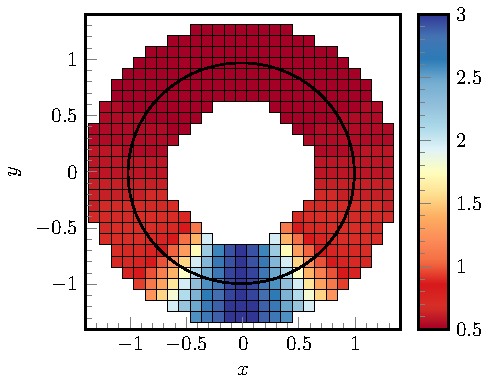
\includegraphics{figs/cylindermesh}
\includegraphics{figs/cylinderprofile}
\caption{(Left) Mesh and closest point domain. (Right) thin film profiles at different times. Numerics are for $\delta = 0.1$, $\Bo = 100$, $\Delta t = 10^{-5}$, $\Delta x = \Delta y = 0.1$ and plotted every $400$ timesteps. The inset displays the thin film height at the top, $\theta = 0$ as a function of time, with the circles indicating numerical results and the solid line for the asymptotic behaviour.}
\end{figure*}

As shown in \cite{trinh_2014}, a simple estimate can be developed for the draining speed near the top of the cylinder. If we assume the film takes the form of a uniform profile near $\theta = 0$, a dominant balance indicates $h_t \sim -\Bo [\theta h^3/3]_\theta$ for which $h \sim [1 - (2\Bo/3) t]^{-1/2}$ is a solution.

\subsection{Axial flow on 3D capped cylinder}

\subsection{Flow on a sphere}
\subsection{Flow on a torus}

\section{Implementation of the full surface curvature}

In the following $S$ denotes the surface of the curved substrate.
Moreover, we use
\begin{enumerate}
\item the convention $\hat{x}$ denotes a point on the substrate surface $\hat{x} \in S$, $x \in \Real^3$ denotes a point in the surrounding
			(which may or may not happen to be on the substrate surface)
	\item The function $d$ denotes the signed Euclidean distance to $S$. 
			$d$ satisfies the Eikonal equation
			\begin{align}
				|\nabla d|^2 &= 1.
			\end{align}
			Because of that property the gradient gives the normal field $N(\hat{x}) = \nabla d(\hat{x})$.
			The sign convention for $d$ is such that $N$ points to that side of $S$ where the thin film is.
	\item $\cp(x)$ denotes the closest point of $x$ on the surface.
	\item The function $h(t,\hat{x})$ gives the height of the thin film.
			For an $\hat{x}$ the corresponding point on the free surface is given by
			\begin{align}
				\hat{x} + h(t,\hat{x}) \; N(\hat{x})
			\end{align}
\end{enumerate}
	
Now, we are interested in the free surface curvature. This quantity is easy to compute given a level set function $\varphi$ which
vanishes on the free surface, and is positive above the free surface and negative below the free surface.
Construction of such a $\varphi$: 
if $x$ is somewhere in space, then $\hat{x} := \cp(x)$ gives its closest point on the surface.
Now, if
\begin{enumerate}
	\item $d(x) > h(t,\cp(x))$, then $x$ is above the free surface
	\item $d(x) = h(t,\cp(x))$, then $x$ is on the free surface
	\item $d(x) < h(t,\cp(x))$, then $x$ is below the free surface.
\end{enumerate}

Thus
\begin{align}
	\varphi(x) &:= d(x) - h(t,\cp(x))
\end{align}
is such a level set function.
Let
\begin{align}
	\hat{h}(t,x) &:= h(t,\cp(x)).
\end{align}
That is because in the closest point method we work with the closest point extension of $h$ which is exactly $\hat{h}$.
So, we can use 
\begin{align}
	\varphi(x) &= d(x) - \hat{h}(t,x)
\end{align}

The free surface curvature $\kappa_f$ is given by
\begin{align}
	\kappa_f &= \Div \left( \frac{\nabla \varphi}{|\nabla \varphi|} \right) &  \text{for  } \varphi(x) &= 0.
\end{align}

For the closest point iteration, this would mean: at each time step do
\begin{enumerate}
	\item set $\varphi(x) = d(x) - \hat{h}(t,x)$
	\item find $\nabla \varphi$ and normalize
	\item find divergence and set $\kappa_f = \Div \left( \frac{\nabla \varphi}{|\nabla \varphi|} \right)$
	\item then perform update to get $\hat{h}(t + \tau,x)$
\end{enumerate}
\bigskip

Remarks:
\begin{enumerate}
	\item	$\kappa_f$ gives a function defined on the surrounding space and in order to get the exact free surface curvature we have to evaluate at the free surface, i.e.
			if $\hat{x}$ is on the surface we have to evaluate at $\hat{x} + h(t,\hat{x}) \; N(\hat{x})$.
			Under the usual assumption that $h$ is small, one performs (implicitly) the usual linearization
			\begin{align}
				\kappa_f(\hat{x} + h(t,\hat{x}) \; N(\hat{x})) &\approx \kappa_f(\hat{x})
			\end{align}
			The only simplification here is with regard to the domain of $\kappa_f$, not the range of $\kappa_f$.
	\item Everything relies on the fact for $\hat{x} \in S$ the point $\hat{x} + h(t,\hat{x}) \; N(\hat{x})$ is on the free surface.
			This assumption can only be true if $h$ stays (for all times) smaller than the smallest distance value such that $\nabla d$ is defined.
			If for some reason $h$ fails to obey this rule, the function $\varphi$ defined above need not obey the explanation given above
			and thus $\kappa_f$ as computed from $\varphi$ might be meaningless.
	\item Because of the usually applied nondimensionalization, the function $\varphi$ defined above needs an appropriate scaling!!!
			Dear modeller, tell me how to scale.
\end{enumerate}

\section{Discussion}

\begin{itemize}
\item We have shown how the general thin film equations over an arbitrary curved substrate can be solved using the cloest point method
\item Most notably, this provides an extremely effective and simple method for studying thin films; numerous advantages over a finite difference approach, which is incapable of studying geometries that are not so easily parameterized (e.g. sphere)
\item Future challenges include: implicit time stepping schemes; how to better resolve singular behaviour such as rupturing, contact lines, etc.; what is the penalty for violating physical principles (e.g. fluid height going negative?)
\item Ability to use the full free surface curvature is a powerful idea
\end{itemize}


\acknowledgements{We thank P.D. Howell and H.A. Stone for many helpful discussions}

\newpage


\begin{appendix}

\section{Differential geometry}

The metric and shape of the substrate, $\rs(s_1, s_2)$, are described using the first and second fundamental forms, $\{\E, \F, \G, \L, \M, \N\}$. Using derivative notation, $\rs_i = \partial_{s_i} \rs$, we define
\begin{equation}\label{funform}
\begin{alignedat}{6} 
\E &= \rs_1 \cdot \rs_1, 
&\quad \F &= \rs_1 \cdot \rs_2, 
&\quad \G &= \rs_2 \cdot \rs_2, \\
\L &= \rs_{11} \cdot \n,
&\quad \M &= \rs_{12} \cdot \n,
&\quad \N &= \rs_{22} \cdot \n,
\end{alignedat}	
\end{equation}
%
where the unit outward normal is 
\begin{equation}
\n = \frac{\rs_1 \wedge \rs_2}{|\rs_1 \wedge \rs_2|}.
\end{equation}
%
The two principal curvatures are the two eigenvalues of 
\begin{equation}
	\begin{pmatrix}
	\L & \M \\ \M & \N
	\end{pmatrix} = \lambda 
	\begin{pmatrix}
	\E & \F \\ \F & \G \end{pmatrix}.
\end{equation}
%
However, as we have chosen for $(s_1, s_2)$ to correspond to directions of principal curvature, then $F \equiv 0 = \M$, and the two principal curvatures are  
\begin{equation}
\kappa_1 = \frac{\L}{\E}, \qquad \kappa_2 = \frac{\N}{\G},	
\end{equation}
%
Note that the unit vectors for $(s_1, s_2)$ system are then given by 
\begin{equation}
\ea = \frac{\rs_1}{\|\rs_1\|} = \frac{\rs_1}{\E^{1/2}}, \qquad
\eb = \frac{\rs_2}{\|\rs_2\|} = \frac{\rs_2}{\G^{1/2}}, 
\end{equation}
%
for the associated metric coefficients $a_1 = \|\rs_1\| = \E^{1/2}$ and $a_2 =  \|\rs_2\| = \G^{1/2}$. We have thus completely described the substrate parameterization. 

For the free surface parameterization, $\r = \rs + \ep h \n$, we denote the fundamental forms with tildes $\{\t{E}, \t{F}, \t{\G}, \t{\L}, \t{\M}, \t{\N}\}$, and use the analogous definitions to \eqref{funform} with $\rs$ replaced by $\r$ and $\n$ replaced by $\t{\n}$. This gives, for the first fundamental forms, 
\begin{equation} \label{tEG}
\begin{aligned}
\t{\E} &= \E(1 - \ep h \kappa_1)^2 + \Oh(\ep^2), \quad \F = \Oh(\ep^2) \\
\t{\G} &= \G(1 - \ep h \kappa_2)^2 + \Oh(\ep^2).
\end{aligned}	
\end{equation}
%
Effectively, we wish to calculate the free-surface curvature to $\Oh(\ep^2)$. This is 
\begin{equation} \label{tK}
\K = \frac{\t{\L}}{\t{\E}} + 
\frac{\t{\N}}{\t{\G}} + \Oh(\ep^2) \sim \frac{\r_{11} \cdot \t{\n}}{\t{\E}} + 
\frac{\r_{22} \cdot \t{\n}}{\t{\G}},
\end{equation}
%
however, a mistake that appears in the work of \cite{myers_2002} is due to the use of the substrate normal, $\n$, in the above expression rather than the free-surface normal. 

Note that since $(s_1, s_2, s_3)$ form an orthogonal system, we have $\rs_i \cdot \n = 0$. Consequently, differentiation implies $\rs_{ij} \cdot \n = -\rs_i \cdot \n_j$. This fact allows us to prove that 
\begin{equation} \label{n12}
	\begin{aligned}
\n_1 &= -(\L/\E)\rs_1 = -\kappa_1 \rs_1, \\
\n_2 &= -(\N/\G)\rs_2= -\kappa_2 \rs_2.	
	\end{aligned}
\end{equation}


 Next, we note that the free surface normal is 
\begin{equation} \label{nexpand}
\t{\n} = \frac{\t{\r}_{11}\wedge \t{\r}_{22}}{\|\t{\r}_{11}\wedge \t{\r}_{22}\|}
= \n - \ep\Bigl[\frac{h_2}{\G} \rs_2 + \frac{h_1}{\E} \rs_1 \Bigr] + \Oh(\ep^2).		
\end{equation}
%
By differentiating $\rs_i \cdot \rs_j$ and using $\F = \rs_1 \cdot \rs_2 = 0$. We may obtain the two identities,
\begin{equation} \label{Rijk}
(\rs_{11} \cdot \rs_i) = -\frac{(-1)^{i}\E_i}{2}, \quad
(\rs_{22} \cdot \rs_i) = \frac{(-1)^i\G_i}{2}.
\end{equation}
%
Using \eqref{nexpand} and \eqref{Rijk}, this allows us to write
\begin{equation} \label{Rijn}
\begin{aligned}
\rs_{11} \cdot \t{\n} &= \L + \ep \left[\frac{h_2\E_2}{\G} - \frac{h_1\E_1}{\E}\right]\\
\rs_{22} \cdot \t{\n} &= 
\N + \ep \left[\frac{h_1\G_1}{\E} - \frac{h_2\G_2}{\G} \right]
\end{aligned}
\end{equation}

We may now calculate 
\begin{equation}
\begin{aligned}
\t{\L} &= (\rs_{11} \cdot \t{n}) + \ep \partial_{s_1}^2 (h\n) \cdot \n + \Oh(\ep^2), \\
\t{\N} &= (\rs_{11} \cdot \t{n}) + \ep \partial_{s_2}^2 (h\n) \cdot \n + \Oh(\ep^2).
\end{aligned}	
\end{equation}
%
In both lines, the first term follows from \eqref{Rijn} and the centre term can be expanded using the fact that $(\rs_1, \rs_2, \n)$ form an orthogonal triad and applying \eqref{n12}. This yields
\begin{equation} \label{tLN}
\begin{aligned}
\t{\L} &\sim \L + \ep(h_{11} - h\kappa_1^2 \E) + \ep \left[\frac{h_2\E_2}{\G} - \frac{h_1\E_1}{\E}\right] \\
\t{\N} &\sim \N + \ep(h_{22} - h\kappa_2^2 \G) + \ep \left[\frac{h_1\G_1}{\E} - \frac{h_2\G_2}{\G}\right] 
\end{aligned}	
\end{equation}
%
and corrects the formulae below eqn. (14) in \cite{myers_2002} to include the additional square bracketted terms. Finally, combining \eqref{tEG}, \eqref{tK}, and \eqref{tLN} gives for the mean curvature
\begin{equation}
\K = (\kappa_1 + \kappa_2) + \ep h (\kappa_1^2 + \kappa_2^2) + \ep \slap h + \Oh(\ep^2),
\end{equation}
%
where we have used the 
\begin{equation}
\slap h = \frac{\left[\pd{}{s_1} \left(\sqrt{\frac{\G}{\E}}\pd{h}{s_1}\right)
+ \pd{}{s_2} \left(\sqrt{\frac{\E}{\G}}\pd{h}{s_2}\right)\right]}{\sqrt{\E\G}}.
\end{equation}

Note finally that the scale factors are 
\begin{align}
m_1^2 &= E(1 - \ep h \kappa_1)^2 \\
m_2^2 &= G(1 - \ep h \kappa_2)^2 \\
m_3^2 &= 1.
\end{align}



% \section{Differentiation formulae}

% Gradient operators:
% \begin{subequations}
% \begin{alignat}{3}
% \nabla &= \sum_i \frac{e_i}{m_i} \pd{}{q_i}, \\
% \nabla \cdot \mb{u} &= \frac{1}{m_1 m_2 m_3} \left[ \pd{}{q_1} ( m_2 m_3 u_1) + \pd{}{q_2} ( m_1 m_3 u_2) + \pd{}{q_3} ( m_1 m_2 u_3) \right] = 0, \\
% &\qquad = \frac{1}{m_1 m_2 m_3} \sum_{i=0}^3 \pd{}{q_i} ( m_j m_k u_i), \label{div} \\
% \nabla^2 &= \frac{1}{m_1 m_2 m_3} \left[ \pd{}{q_1} \left( \frac{m_2 m_3}{m_1} \pd{}{q_1}\right) 
% + \pd{}{q_2} \left( \frac{m_3 m_1}{m_2} \pd{}{q_2}\right) 
% + \pd{}{q_3} \left( \frac{m_1 m_2}{m_3} \pd{}{q_3}\right)\right], \\
% &\qquad = \frac{1}{m_1 m_2 m_3} \sum_{i=0}^3  \pd{}{q_i} \left( \frac{m_j m_k}{m_i} \pd{}{q_i}\right).
% \end{alignat}
% \end{subequations}

% \noindent Derivatives of unit vectors are \cite[p.483]{happel_book}
% \begin{alignat}{3} 
% \pd{\mb{e}_i}{x_j} &= \frac{\mb{e}_j}{m_i} \pd{m_j}{x_i}  \\ 
% \pd{\mb{e}_i}{x_i} &= -\frac{\mb{e}_j}{m_j} \pd{m_i}{x_j} - 
% \frac{\mb{e}_k}{m_k} \pd{m_i}{x_k}.
% \end{alignat}

% \noindent or simply \cite[p.241]{roy_2002}:
% \begin{equation}
% \pd{\mb{e}_i}{x_j} = \frac{\mb{e}_j}{m_i} \pd{m_j}{x_i} - \delta_{ij} \sum_{k=1}^3 \frac{\mb{e}_k}{m_k} \pd{m_i}{x_k}.
% \end{equation}

% \subsection{Surface quantities}
% \begin{equation} \label{surfdiv}
% \nabla_s \cdot (q_1 \ea + q_2 \eb) = \frac{1}{a_1 a_2} \left[ \pd{}{x_1} (a_2 q_1) + \pd{}{x_2} (a_1 q_2) \right].
% \end{equation}

% \begin{equation}
% \nabla_s = \pd{}{x_1} \frac{\ea}{a_1} + \pd{}{x_2} \frac{\eb}{a_2}.
% \end{equation}

% \begin{equation}
% \nabla_s^2 = \frac{1}{a_1 a_2} \left[ \pd{}{x_1} \left( \frac{a_2}{a_1} \pd{}{x_1}\right) + \pd{}{x_2} \left(\frac{a_1}{a_2} \pd{}{x_2}\right)\right].
% \end{equation}


%In order to derive the tangential stress, we will need two vectors that span the tangent plane at the point $(x_1, x_2, n)$. If $\mb{t}$ is an arbitrary tangent, then $\mb{n} \cdot \mb{t} = 0$. This gives us two tangent vectors: 
%\begin{align}
%\mb{t}_1 
%&= \frac{n_2 \ea - n_1 \eb}{\sqrt{n_1^2 + n_2^2}} 
%= \frac{\left[-\frac{1}{m_2} \pd{h}{x_2} \ea + \frac{1}{m_1} \pd{h}{x_1} \eb\right]}
%{\sqrt{\left(\frac{1}{m_2} \pd{h}{x_2}\right)^2 + \left(\frac{1}{m_1} \pd{h}{x_1}\right)^2}}  \\
%\mb{t}_2 
%&= \frac{n_3 \ea - n_1 \ec}{\sqrt{n_1^2 + n_3^2}} 
%= \frac{\left[ \ea + \frac{1}{m_1} \pd{h}{x_1} \ec\right]}
%{\sqrt{1 + \left(\frac{1}{m_1} \pd{h}{x_1}\right)^2}} 
%\end{align}



%\noindent For the two tangents that span the tangent plane, recall that the position vector is given by $\mb{r} = x_1 \ea + x_2 \eb + n \ec$. For this, we need to use the formulae (\ref{}) to differentiate the unit vectors. We get
%\begin{gather}
%\pd{\ea}{x_1} = -\eb m_2 \pd{}{x_2} \left(\frac{1}{m_1}\right) - \ec \pd{}{n} \left(\frac{1}{m_1}\right) \\
%\pd{\ea}{x_2} = \eb m_1 \pd{}{x_1} \left(\frac{1}{m_2}\right) \\ 
%\pd{\ea}{x_3} = 0 \\ 
%\pd{\ec}{x_1} = \pd{\ec}{x_2} = 0, \quad \pd{\ec}{n} = 1 \\ 
%\end{gather}
%
%\begin{align}
%\pd{\mb{r}}{x_1}  &= \ea + x_1 \pd{\ea}{x_1} + x_2 \pd{\eb}{x_1} + \pd{h}{x_1} \ec  \\ 
%&= \ea\left[ 1 + x_2 m_2 \pd{m_1^{-1}}{x_2}\right] + \eb \left[ -x_1 m_2 \pd{m_1^{-1}}{x_2}\right]
%+ \ec \left[\pd{h}{x_1} - x_1 \pd{m_1^{-1}}{n}\right]. 
%\end{align}

\end{appendix}
% \bibliographystyle{plain}
\bibliographystyle{/Users/trinh/Dropbox/documents/bib/styles/apsrev4-1-edit}
\bibliography{/Users/trinh/GoogleDrive/papers/philmaster}


\end{document}

